\documentclass[oneside]{VUMIFPSkursinis}
\usepackage{algorithmicx}
\usepackage{algorithm}
\usepackage{algpseudocode}
\usepackage{amsfonts}
\usepackage{float}
\usepackage{amsmath}
\usepackage{bm}
\usepackage{caption}
\usepackage{color}
\usepackage{float}
\usepackage{graphicx}
\usepackage{listings}
\usepackage{subfig}
\usepackage{tabularx}
\usepackage{wrapfig}
\newcolumntype{P}[1]{>{\centering\arraybackslash}p{#1}}
\usepackage[%  
    colorlinks=true,
    linkcolor=black
]{hyperref}
\university{Vilniaus universitetas}
\faculty{Matematikos ir informatikos fakultetas}
\department{Programų sistemų katedra}
\papertype{}
\title{Virtualios ir realios mašinos modelis}
\titleineng{Virtual and real machine model}
\status{2 kurso 3 grupės studentai}
\author{Matas Savickis}
\secondauthor{Justas Tvarijonas}  
\thirdauthor{Greta Pyrantaitė}   
\supervisor{Mantas Grubliauskas Lekt.}
\date{Vilnius – \the\year}


\bibliography{bibliografija}

\begin{document}
\maketitle
\tableofcontents

\section{Reali mašina}
\begin{figure}[H]
		\centering	
	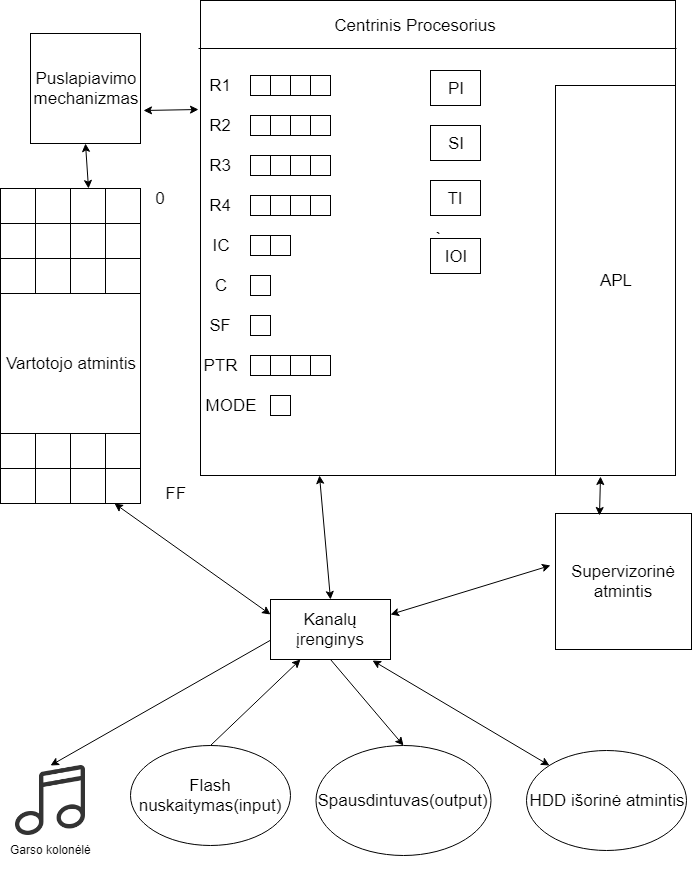
\includegraphics[width=18cm,height=20cm,keepaspectratio]{RealiMasina.png}
	\caption{Reali mašina}
	\label{fig:Reali mašina}
\end{figure}

\pagebreak

\subsection{Techninės įrangos elementai sudarantys realią mašiną}
\begin{itemize}
	\item{Centrinis procesorius}
	\item{Vartotojo atmintis}
	\item{Supervizorinė atmintis}
	\item{Išorinė atmintis}
	\item{Duomenų perdavimo kanalas}
	\item{Įvedimo įrenginys - flash atmintinis}
	\item{Išvedimo įrenginys - spausdintuvas}
	\item{Papildomas išvedimo įrenginys - garso kolonėlė}
	\item{Puslapiavimo mechanizmas}
\end{itemize}

\subsection{Centrinis procesorius}
	Centrinio procesoriaus paskirtis yra skaityti komandas iš atminties ir jas interpretuoti. Procesorius gali dirbti dviem rėžimais - supervizoriaus ir vartotojo. Supervizoriaus rėžime komandos yra apdorojamos aukšto lygio procesoriaus. Komandos vykdomos supervizoriaus režime yra skirtos operacinės sistemos funkcionavimui palaikyti. Procesorius persijungia į šį rėžimą pertaukimais arba sisteminiais kreipiniais.
\subsection{Procesoriaus registrai}
\begin{itemize}
	\item{R1, R2, R3, R4 - 4 baitų bendros paskirties registrai}  
	\item{IC - 2 baitų komandų skaitiklis}
	\item{C - 1 baito loginis registras (TRUE arba FALSE)}
	\item{SF - 1 baito požymių registras CF ZF SF IF OF XXX - carry flag, zero flag, sign flag, interupt flag, overflow flag}
	\item{PTR - 4 baitų puslapių lentelės registras(naudojamo puslapių lentelės adresas)}
	\item{MODE - registras, kurio reikšmė nusako procesoriaus darbo režimą(supervizorinis, vartotojo)}
	\item{PI - programinių pertraukimų registras}
	\item{SI - supervizorinių pertraukimų registras}
	\item{TI - taimerio registras}
	\item{IOI - 2 baitų įvedimo ir išvedimo pertraukimų registras}
\end{itemize}

\subsection{Atmintys}
Pagrindinę realios mašinos atmintį dalinasi vartotojo ir supervizorinė atmintis. Kaskart sukuriant naują virtualią mašiną panaudojama dalis realios mašinos atminties. Atminties dydis 256 blokų po 16 žodžių. Žodžio ilgis 4 baitai. Supervizorinę atmintį naudoja aukšto lygio procesorius, tačiau šios atminties savo rašomoje programoje nenaudosim. Taip pat yra išorinė atmintis kietojo disko pavidalu.

\subsection{I/O}
Komandų įvedimui naudojamas ,,flash atmintinių" nuskaitymo įrenginys. Išvedimui naudojamas spausdintuvas. Abu šie įrenginiai tėra modeliai ir didelio skirtumo nedarys.

\subsection{Puslapiavimo mechanizmas}
Puslapiavimo mechanizmas yra metodas skirtas virtualios atminties adreso parodymui į realios atminties adresą. Kiekvienai virtualiai mašinai skiriama 16 atminties blokų. Sukuriant virtualią mašiną sukuriama puslapių lentelė. Naudojamas PTR(4 baitų a0,a1,a2,a3) registras kuriame laikomas puslapių lentelės adresas. Baitai a0 ir a1 yra nenaydojami, o a2 * 16 + a3 žymi puslapių lentelės adresą. Dabar galime pateikti formulę, kuri virtualiam adresui x1x2 gražina realų adresą: Realus adresas = 16*[16*(16 * a2 + a3) + x1] + x2.
\subsection{Garso kolonėlė}
Vartotojui įvedus atitinkamą komandą kompiuterio garso kolonėlė supypsi x1 kartų.
\subsection{Pertraukimų mechanizmas}
Vykdant komandą virtualioje mašinos gali kilti pertraukimai, tuo atvėju nustatoma atitinkamu registrų reikšė ir nutraukiamas komandos vykdymas. Kviečiant test() metodą, patikrinama ar įvyko pertraukimas, jam įvykus nutraukiamas virtualios mašinos darbas ir kviečiamas metodas Test(), kuris apdorojo pertraukimą. Apdorojus pertraukimą sprendžiama ar grąžinti darbą atgal virtualiai mašinai. Galimi pertraukimai:
\begin{itemize}
\item Operacijos GD, PD, PY ir HALT iššauks supervizorinius pertraukimus. SI = 1 - komanda
GD, SI = 2 - komanda PD, SI = 3 - komanda PY, SI = 4 – komanda HALT.
\item Programiniai pertraukimai:PI = 1 – neteisingas adresas, PI = 2 – neteisingas operacijos
kodas, PI = 3 – neteisingas priskyrimas, PI = 4 – perpildymas (overflow).
\item Esant TI = 0 bus fiksuojamas taimerio pertraukimas.
\end{itemize}
\subsection{Timerio mechanizmas}
Vygdant virtualią mašiną kas komandą mažinama timerio registro reikšmė, jai pasiekus 0 įvyksta pertraukimas, o jį apdorojus timerio reikšmė nustatoma 10.
\subsection{Duomenų perdavimo kanalai}
Skirti I/O ir atminties valdymui.Modelyje yra vienas kanalas kuriam galima padaryti skirtingas paskirtis: rašyti, skaityti arba abu. Duomenys eina per kanalą ir pats kanalo įrenginys juos nukreipia į reikiamą kryptį ir pasako kiek duomenų gali pasiimti o kiek reikia nukirpti. Kanalų įrenginio registrai:\newline
\newline SB: Žodžio, nuo kurio kopijuosime numeris.
\newline DB: Žodžio, į kurį pradėsime rašyti numeris
\newline ST: Objekto, iš kurio kopijuosime, numeris
\newline 1. Vartotojo atmintis;
\newline 2. Supervizorinė atmintis;
\newline 3. Išorinė atmintis;
\newline 4. Įvedimo srautas;
\newline DT: Objekto, į kurį kopijuosime, numeris
\newline 1. Vartotojo atmintis;
\newline 2. Supervizorinė atmintis;
\newline  3. Išorinė atmintis;
\newline 4. Išvedimo srautas; 

\section{Virtuali mašina}

\subsection{Funkcija}
Virtuali mašina yra skirta paslepti realios mašinos sudėtingumą ir suteikti vartotojui instrukcijų sąrašą su kuriuo jis galėtų dirbti. Todėl operacinės sistemos paskirtis ir yra paslėpti realią mašiną ir duoti mums virtualią. Virtuali mašina taip pat suteikia darbų pasidalijimą kurio dėka galima paleisti kelias virtualias mašinas ir tokiu būdu ant kiekvienos iš jų atlikti skirtingas užduotis.

 \subsection{Modeliuojamos virtualios mašinos loginių komponentų aprašymas}
	\subsubsection{Atmintis}
	\begin{figure}[H]
		\centering	
	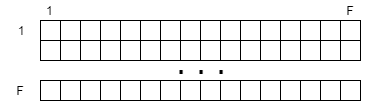
\includegraphics[width=18cm,height=20cm,keepaspectratio]{VMAtmintis.png}
	\caption{Virtualios mašinos atmintis}
	\label{fig:Virtualios mašinos atmintis}
\end{figure}

	Virtualios mašinos atmintis susideda iš 16 blokų po 16 žodžių iš viso 256 žodžiai po 4 baitus arba 32 bitus. Naudosime registrą PTR(4 baitai a0 a1 a2 a3) kuriame laikomas adresas į puslapių lentelę. Baitai a0 ir a1 nenaudojami, o a2 * 16 + a3 žymi puslapių lentelės adresą. Dabar galime pateikti formulę, kuri virtualiam
adresui x1x2 gražina realų adresą:
Realus adresas = 16*[16*(16 * a2 + a3) + x1] + x2

	\subsubsection{Procesorius}
\begin{figure}[H]
		\centering	
	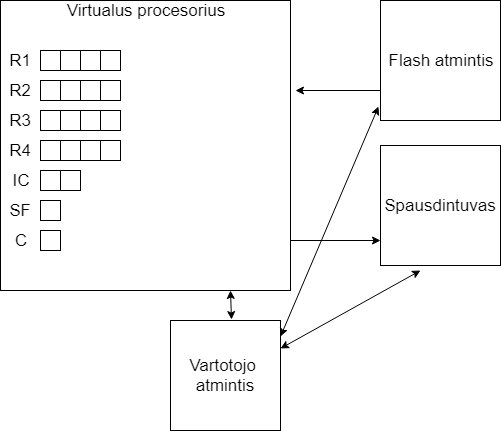
\includegraphics[width=18cm,height=20cm,keepaspectratio]{VMProcesorius.png}
	\caption{Virtualios mašinos procesorius}
	\label{fig:Virtualios mašinos procesorius}
\end{figure}
Registrai:
\begin{itemize}
	\item{R1...R4 - Bendros paskirties registrai}
	\item{IC - komandos skaitliukas, rodo sekančios komandos adresą }
	\item{SF - status flagas rodantis programos būseną}
	\item{C - loginis registras(TRUE arba FALSE)}

\end{itemize}
	\subsubsection{Virtualios mašinos komandų sistema}
Kiekvieną virtualios mašinos komandą sudaro 4B, tačiau priklausomai nuo komandos ne visi
baitai turi būti užimti – jie gali būti ir tušti.
Komandos:
\begin{enumerate}
\item Duomenų persiuntimui iš atminties į registrus ir atvirkščiai:
\begin{enumerate}
\item  LR – Load Register – iš atminties baito x1x2 persiunčia į registrą R:
LR x1x2 =) R:=[x1x2];
\item SR – Save Register – iš registro R persiunčia į atminties baitą x1x2:
SR x1x2 =) [x1x2]:=R;
\end{enumerate}
\item Duomenų sukeitimui tarp registrų:
\begin{enumerate}
\item RR – sukeičia registro R ir R2 reikšmes:
RR =) R:=R+R2, R2=R-R2, R=R-R2;
\end{enumerate}
\item Aritmetinės komandos:
\begin{enumerate}
\item AD – suma – prie esamos registro R reikšmės prideda reikšmę esančią x1x2 atminties
baite, rezultatas patalpinamas registre R:
AD x1x2 =) r1:=r1+[x1x2];
\item SB – atimtis – iš esamos registro R1 reikšmės atimama reikšmė esanti x1x2 atminties
baite, rezultatas patalpinamas registre R:
SB x1x2 =) r1:=r1-[x1x2];
\item CR – palyginimas – esamą registro R reikšmė yra lyginama su reikšme esančią x1x2
atminties baite, rezultatas patalpinamas registre C:
CR x1x2 =)
if r1>[x1x2] then cf:=0, zf:=0;
if r1=[x1x2] then zf:=1;
if r1<[x1x2] then cf:=1;
\item MU x1x2 – daugyba, r1 =r1* [x1x2].
\item DI x1x2 – dalyba, r1=r1/[x1x2] , r2=r1\%[x1x2].
\end{enumerate}
\item Valdymo perdavimo:
\begin{enumerate}
\item PY x1 - Garso kolonėlė supypsi x1 kartų.
\item PYC - Patikrina garso kolonėlės užimtumą.(1 - užimta , 0 - laisva).
\item JU – besąlyginio valdymo perdavimas – valdymas perduodamas adresu 16*x1+x2:JU x1x2 =) IC:=16*x1+x2;
\item JG – sąlyginio valdymo perdavimas (jeigu daugiau) – valdymas perduodamas jeigu SF bitai ZF == 0 ir SF == OF. Valdymas perduodamas adresu 16*x1+x2:JG x1x2 =) If ZF == 0 AND SF == OF then IC:= 16*x1+x2;
\item JE – sąlyginio valdymo perdavimas (jeigu lygu) – valdymas perduodamas jeigu SF bitas ZF == 1.Valdymas perduodamas adresu 16*x1+x2:JE x1x2 =) If ZF == 1 then IC:= 16*x1+x2;
\item JL – sąlyginio valdymo perdavimas (jeigu mažiau) – valdymas perduodamas jeigu SF bitai SF ir OF nelygūs, valdymas perduodamas adresu 16*x1+x2:JL x1x2 =) If SF != OF then IC:= 16*x1+x2;
\end{enumerate}
\item Programos pabaigos:
\begin{enumerate}
\item HALT – programos pabaigos komanda.
\end{enumerate}
\item Įvedimo/Išvedimo:
\begin{enumerate}
\item GD – įvedimas – iš įvedimo srauto paima 4 žodžų srautą ir jį įveda į atmintį
pradedant atminties baitu 16*x1+x2:
GD x1x2
\item CKP - patikrina printerio užimtumą.(1 - užimta, 0 - laisva)
\item PD – išvedimas – iš atminties, pradedant atminties baitu 16*x1+x2  paima 4 žodžių
srautą ir jį išveda į ekraną:
PD x1x2
\end{enumerate}
\item Loginės:
\begin{enumerate}
\item AND – r1 := r1 and r2
\item XOR – r1 := r1 xor r2
\item OR - r1 := r1 or r2.
\item NOT - r1 := not r1.
\end{enumerate}
\end{enumerate}
\subsection{Virtualios mašinos bendravimo su įvedimo/išvedimo įrenginiais mechanizmo aprašymas.}
VM duomenis skaito iš flash atminties (realizuotos failu kietajame diske), o rezultatą išveda spausdintuvas. Įvedimą/išvedimą kontroliuoja kanalų įrenginys.
\subsection{Virtualios mašinos interpretuojamojo ar kompiliuojamo vykdomojo failo išeities teksto formatas.}
VM modelio įvedimo įrenginiui pateikiamas programos failas turi būti tokios struktūros: \newline
DATASEG\newline
.\newline
.\newline
.\newline
CODESEG\newline
.\newline
.\newline
.\newline
HALT\newline
Atmintis yra išdėstyta nuosekliai: 128 žodžiai skirti DATASEG (nuo 0 iki 127) ir 128 žodžiai\newline
CODESEG (nuo 128 iki 255).\newline
Programa apskaičiuoja reiškinio „100 + 20 – 80“ reikšmę, bei ją išveda į ekraną.\newline
000 | DATA\newline
001 | 100\newline
002 | 20\newline
003 | 80\newline
004 | Rezu\newline
005 | ltat\newline
009 | as y\newline
00A | ra:\newline
080 | CODE\newline
081 | LR 01\newline
082 | AD 02\newline
083 | SB 03\newline
084 | PD 04\newline
085 | PD 05\newline
086 | PD 06\newline
087 | PD 07\newline
088 | SR 10\newline
089 | PD 10\newline
08A | HALT\newline
0FF |\newline
	\subsection{Modeliuojamos virtualios mašinos loginių komponentų sąryšio su realios mašinos techninės įrangos komponentais aprašymas.}
	Virtualiai mašinai atliekant komandas gali kilti pertraukimai. Jie apdorojami tik tada kai VM
baigia vykdyti komandą.Tuomet reali mašina persijungia iš vartotojo režimo į supervizorinį.\newline
Įvedimo/ Išvedimo veiksmas atliekamas supervizoriniu rėžimu, tam naudojama iniciavimo
operacija StarIO – kuria nustatomi kanalai, jų panaudojimas ir tikrinamas užimtumas.\newline
Norint iš supervizorinio rėžimo į vartotojo rėžimą darbo pratęsimui virtualioje mašinoje
reikalinga pakrauti būsena tam naudojama operacija Slave(plr,c,r,ic) – kur registrų panaudojimas
sutampa su realios mašinos.
	\section{Virtuali mašina operacinės sistemos kontekste}
	Operacinei sistemai turi būti pateikiamas užduočių rinkinys (programa). Tam reikalinga specifinė užduočių pateikimo kalba. Kiekviena užduotis suformuojama kaip failas. Užduotis sudaryta iš pateikiamų duomenų ir rezultatų. Vykdant užduotį ji yra išskaidoma į dalis: užduotis saugoma išorinėje atmintyje, kai ji paruošta vykdymui. Užduotis tiesioginės sąveikos su fiziniais įrenginiais neturi, tik su virtualiais.

\section{Multiprograminės operacinės sistemos modelis}
Šiuolaikinės multiprograminės operacinės sistemos gali vykdyti kelias programos vienu metu. Būtų labai nepatogu jeigu norėdamas atsisiųsti failą iš interneto turėtum laukti ir negalėtum nieko daryti su kompiuteriu. Žinoma multiprogramiškumas nėra abstakcija, kuri realiai neegzistuoja, o tik atrodo, kad keli procesai vyksta vienu metu. Tai palengvina programos vartotojiškuma, tačiau neparodo kaip ištikrūjų veikia operacinė sistema. OS veikimo struktūra bandysime išanalizuoti šiame darbe. 

\subsection{Procesai}
Procesas tai yra programa kuri turi registrų reikšmes, kintamuosius ir virtualų procesorių. Procesas ir programa yra labai panašios savokos, skirtumas tik tas, kad procesas turi savo veiklumo būseną, o programa tėra baitų seka.

\subsection{Procesų būsenos}
Kiekvienas procesas turi jam priskirtą būseną:
\begin{itemize}
\item Pasiruošęs: vienintelis trūkstamas resursas yra procesorius
\item Vykdomas - turi procesorių
\item Blokuotas - prašo resurso (išskyrus procesorių) 
\item Sustabdytas – kito proceso sustabdytas procesas.

\end{itemize}

\begin{figure}[H]
		\centering	
	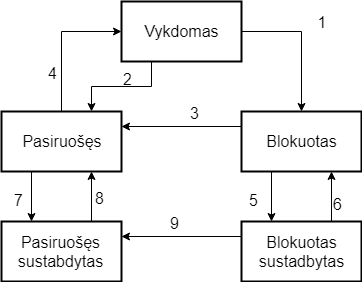
\includegraphics[width=18cm,height=20cm,keepaspectratio]{ProcesuBusenos.png}
	\caption{Virtualios mašinos procesorius}
	\label{fig:Virtualios mašinos procesorius}
\end{figure}

\begin{itemize}
	\item 1. Vykdomas procesas blokuojasi jam prašant ir negavus resurso. 
	\item 2. Vykdomas procesas tampa pasiruošusiu atėmus iš jo procesorių dėl kokios nors priežasties (išskyrus resurso negavimą). 
	\item 3. Blokuotas procesas tampa pasiruošusiu, kai yra suteikiamas reikalingas resursas. 
	\item 4. Pasiruošę procesai varžosi dėl procesoriaus. Gavęs procesorių procesas tampa vykdomu. 
	\item 5. Procesas gali tapti sustabdytu blokuotu, jei einamasis procesas jį sustabdo, kai jis jau ir taip yra blokuotas. 
	\item 6. Procesas tampa blokuotu iš blokuoto sustabdyto, jei einamasis procesas nuimabūseną sustabdytas. 
	\item 7. Procesas gali tapti pasiruošusiu sustabdytu, jei einamasis procesas jį sustabdo,kai jis yra pasiruošęs.
	\item 8. Procesas tampa pasiruošusiu iš pasiruošusio sustabdyto, jei einamasis procesas nuima būseną sustabdytas 
	\item 9. Procesas tampa pasiruošusiu sustabdytu iš blokuoto sustabdyto, jei procesui yra suteikiamas jam reikalingas resursas. 

\end{itemize}

\section{Resursai} Resursai yra tai, dėl ko varžosi procesai.  D÷l resursų trūkumo procesai blokuojasi, gavę reikiamą resursą, procesai tampa pasiruošusiais. Resursus galima skirstyti į: 
\linebreak
\begin{itemize}
	\item  Statinius resursus. Kuriami sistemos kūrimo metu. Tai mašinos resursai, tokie kaip procesorius, atmintis ar kiti resursai, kurie sistemos veikimo metu nėra naikinami. Šie resursai gali būti laisvi, kai nei vienas procesas jų nenaudoja, arba ne, kada juos naudoja vienas ar keli, jei tą resursą galima skaldyti, procesai. 
	\item  Dinaminius resursus. Kuriami ir naikinami sistemos darbo metu. Šie resursai naudojami kaip pranešimai. Kartu su jais gali ateiti naudinga informacija. Kartais šio tipo resursas pats yra pranešimas. Pavyzdžiui, esantis laisvas kanalo resursas žymi, kad bet kuris procesas gali naudotis kanalu. Jei jo n÷ra, procesas priverstas laukti, kol šis resursas taps prieinamu (bus atlaisvintas).
\end{itemize}

\subsection{Resurso primityvai} Kiekvienas resursas turi keturis primityvus
\begin{itemize}
	\item Kurti resursą. Resursus kuria tik procesas. Resurso kūrimo metu perduodami kaip parametrai: nuoroda į proceso kūrėją, resurso išorinis vardas. Resursas kūrimo metu yra: pridedamas prie bendro resursų sąrašo, pridedamas prie tėvo suskurtų resursų sąrašo, jam priskiriamas unikalus vidinis vardas, sukuriamas resurso elementų sąrašas ir sukuriamas laukiančių procesų sąrašas.
	\item Naikinti resursą. Resurso deskriptorius išmetamas iš jo tėvo sukurtų resursų sąrašo, naikinamas jo elementų sąrašas, atblokuojami procesai, laukiantys šio resurso, išmetamas iš bendro resursų sąrašo, ir, galiausiai naikinamas pats deskriptorius
	\item Prašyti resurso. Šį primityvą kartu su primityvu “atlaisvinti resursą” procesai naudoja labai dažnai. Procesas, iškvietęs šį primityvą, yra užblokuojamas ir įtraukiamas į to resurso laukiančių procesų sąrašą. Sekantis šio primityvo žingsnis yra kviesti resurso paskirstytoją.  
	\item Atlaisvinti resursą. Šį primityvą kviečia procesas, kuris nori atlaisvinti jam nereikalingą resursą arba tiesiog perduoti pranešimą ar informaciją kitam procesui. Resurso elementas, primityvui perduotas kaip funkcijos parametras, yra pridedamas prie resurso elementų sąrašo. Šio primityvo pabaigoje yra kviečiamas resursų paskirstytojas. 
 
 
 

\end{itemize}

\section{Planuotojas} Planuotojo paskirtis tvarkyti procesus, iš vienų procesų jis atiima procesorių ir kitiems atiduoda. Jis dirba su branduolio primityvais, procesų sarašu, procesų deskriptoriais ir procesoriaus resurso deskriptoriais. Planuotojas dirbs prioritetų principu, kur kiekvienas procesas turi prioriteto skaičių nuo 1 iki 100. Sisteminiasm procesams skirsime aukštenį prioriteta o vartotojiešiems žemesnį nes taip OS veiks greičiau.

\begin{figure}[H]
		\centering	
	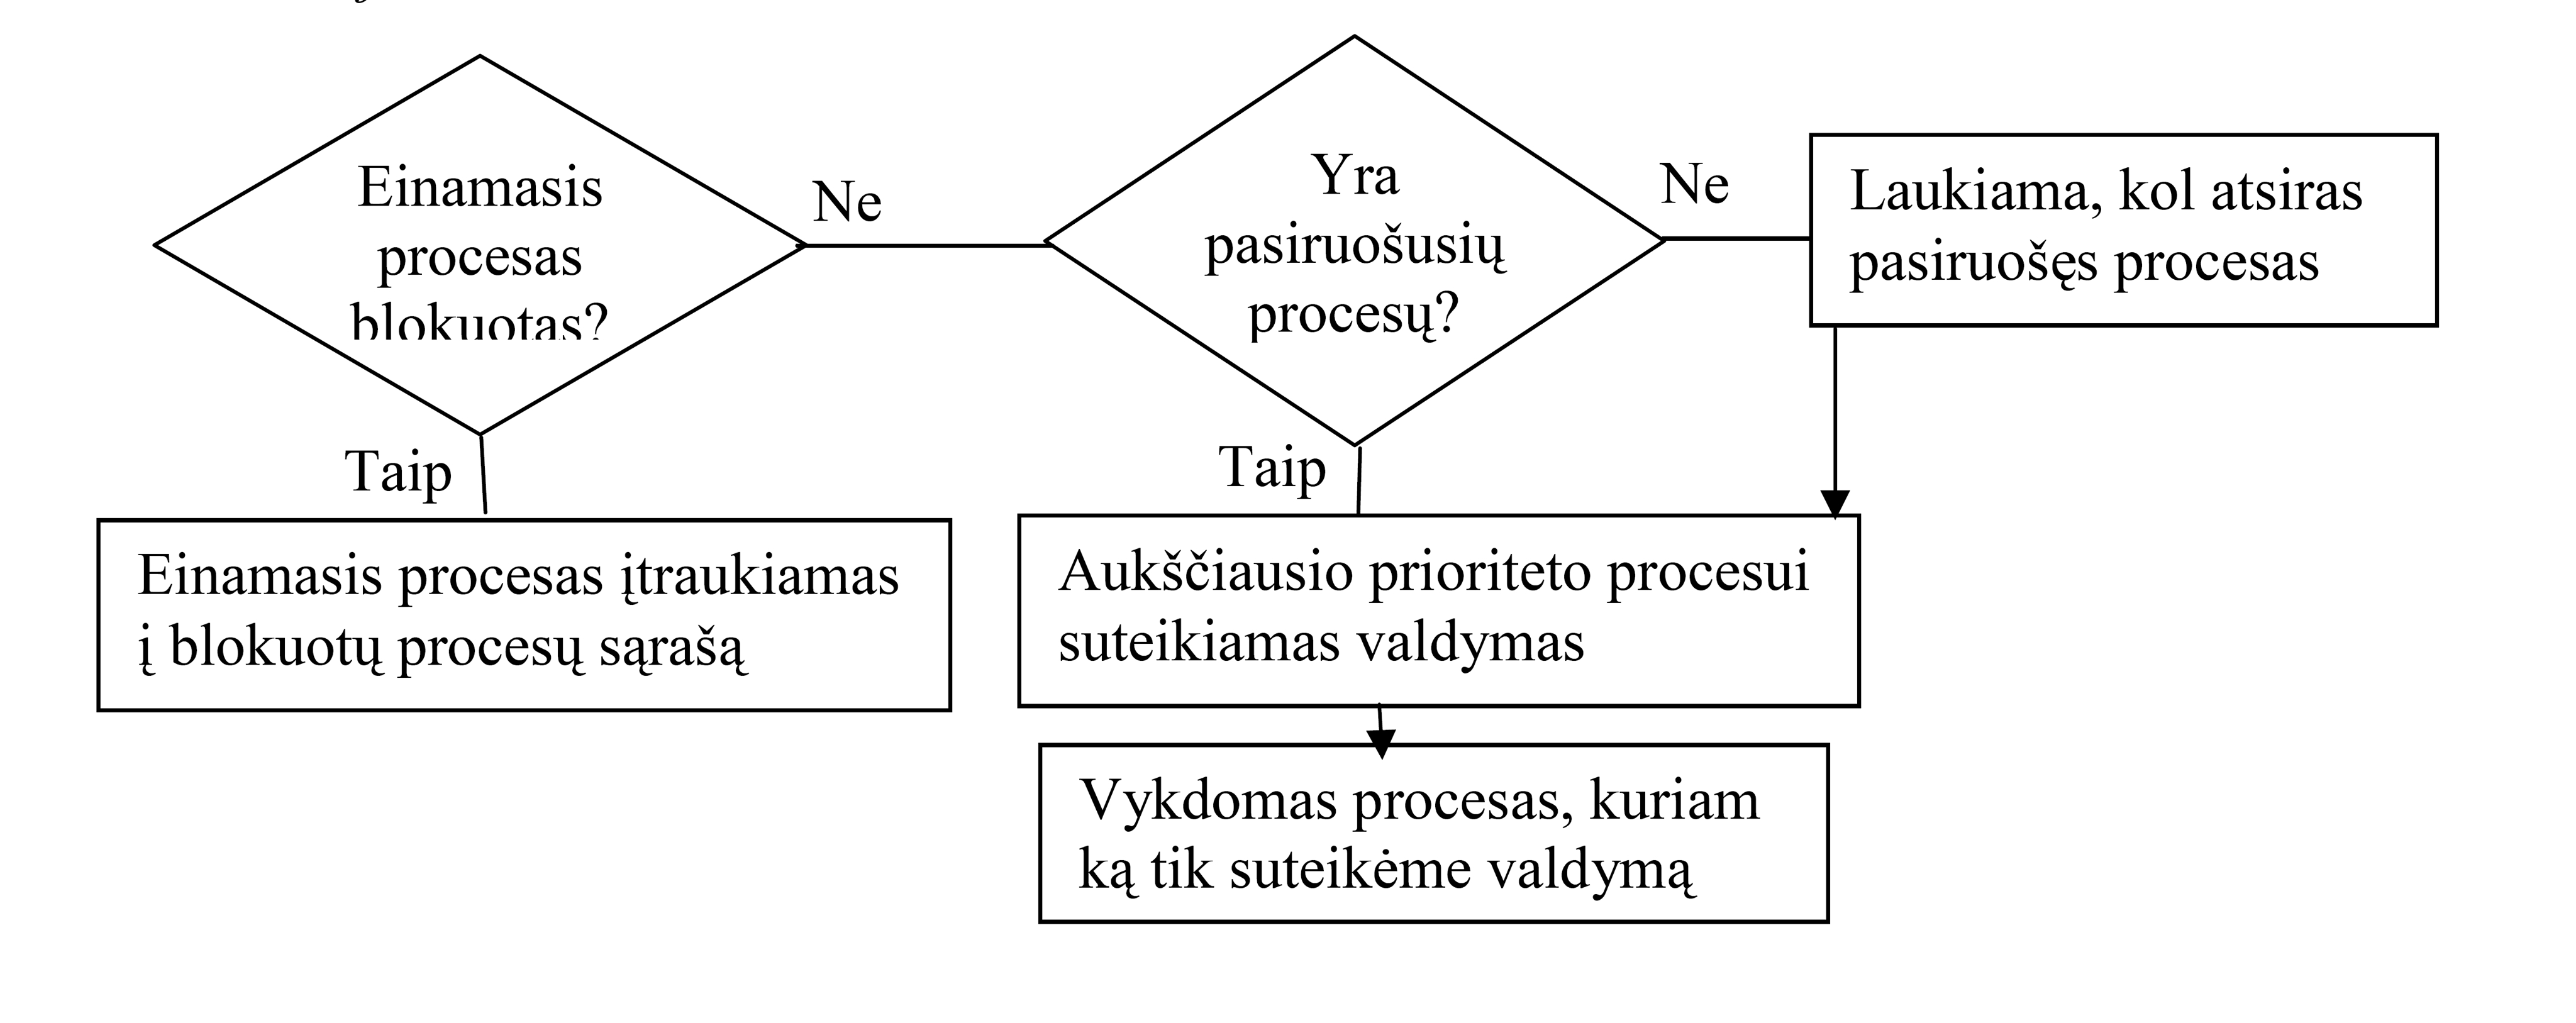
\includegraphics[width=18cm,height=20cm,keepaspectratio]{ProcesuVeikimas.png}
	\caption{Virtualios mašinos procesorius}
	\label{fig:Virtualios mašinos procesorius}
\end{figure}

\section{Procesų hierarchija}

\begin{figure}[H]
		\centering	
	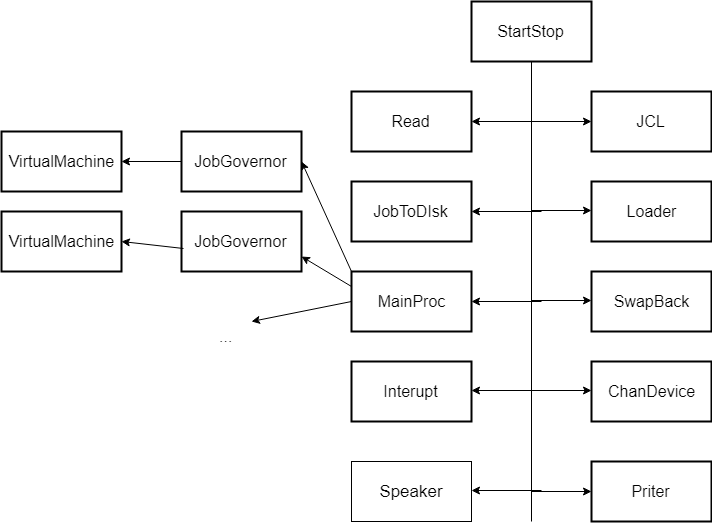
\includegraphics[width=18cm,height=20cm,keepaspectratio]{ProcesuHierarchija.png}
	\caption{Virtualios mašinos procesorius}
	\label{fig:Virtualios mašinos procesorius}
\end{figure}


\subsection{StratStop} Procesas atsakingas už sistemos darbo pradžią ir pabaigą. Proceso paskirtis - sisteminių resursų kūrimas

\begin{figure}[H]
		\centering	
	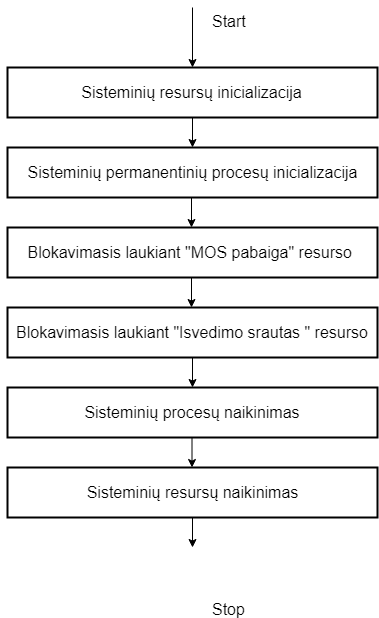
\includegraphics[width=18cm,height=20cm,keepaspectratio]{StartStop.png}
	\caption{Virtualios mašinos procesorius}
	\label{fig:Virtualios mašinos procesorius}
\end{figure}

\subsection{Read} užduoties nuskaitymo iš įvedimoi srauto procesas.

\begin{figure}[H]
		\centering	
	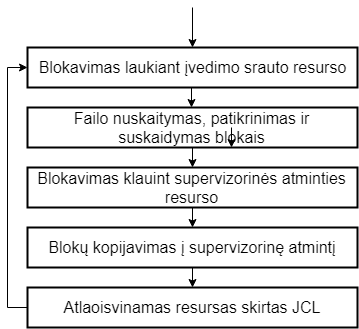
\includegraphics[width=18cm,height=20cm,keepaspectratio]{Read.png}
	\caption{Virtualios mašinos procesorius}
	\label{fig:Virtualios mašinos procesorius}
\end{figure} 

\subsection{JCL} JCL paskirtis - interpretuoti užduoties tekstą, išskiriant duomenis ir paraketrus bei kuriant atitinkamus resursus.

\begin{figure}[H]
		\centering	
	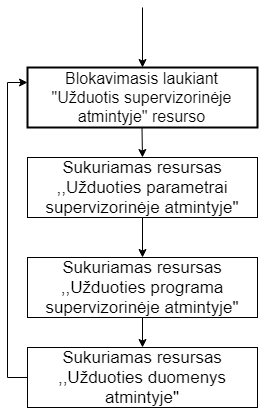
\includegraphics[width=18cm,height=20cm,keepaspectratio]{JLC.png}
	\caption{Virtualios mašinos procesorius}
	\label{fig:Virtualios mašinos procesorius}
\end{figure} 

\subsection{JobToDisk} JobToDisk - procesas skirtas patarlpinti užduotį iš supervizorinės atminties į išorinę atmintį.

\begin{figure}[H]
		\centering	
	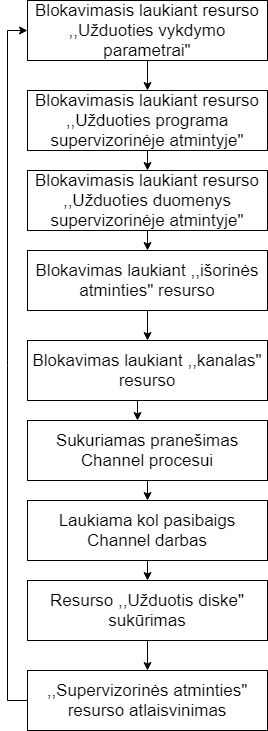
\includegraphics[width=18cm,height=20cm,keepaspectratio]{JobToDisk.png}
	\caption{Virtualios mašinos procesorius}
	\label{fig:Virtualios mašinos procesorius}
\end{figure}

\subsection{MainProc}

MainProc yra procesas atsakingas už užduočių vykdymo paruošimą ir sunaikinimą.
\begin{figure}[H]
		\centering	
	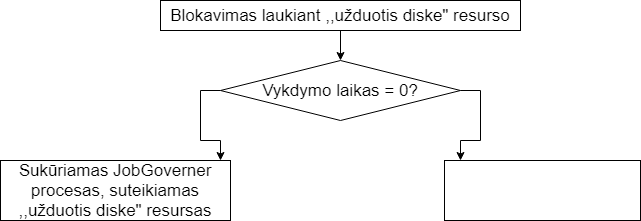
\includegraphics[width=18cm,height=20cm,keepaspectratio]{MainProc.png}
	\caption{Virtualios mašinos procesorius}
	\label{fig:Virtualios mašinos procesorius}
\end{figure}

\subsection{JobGovernor}JobGovernor procesas atsakingas už virtualios mašinos proceso kūrimą ir tvarkantis jos darbą

\section{Proceso deskriptoriaus struktūra}

ID: String                  // išorinis vardas \newline


Resources: LinkedList            // turimų resursų elementų sąrašas \newline

State: String     // {RUN, READY, BLOCK, READYS, BLOCKS} - proceso būsena \newline

ProcessList: Queue       // procesų sąrašas, kuriam šiuo metu priklauso procesas \newline

T: int                // tėvinio proceso vidinis vardas \newline

S: LinkedList     // sūnų sąrašas \newline

Priority: int       // proceso prioritetas \newline

CPU:    // procesoriaus einamoji būsena proceso metu
\begin{itemize}                          
	\item mode: byte     // supervizorinis/vartotojo darbo rėžimas 
	\item entry: int        // (sisteminiam procesui) - įėjimo taškas, nuo kurio bus pratęstas proceso darbas 
	\item r1:  int            // registras, atitinkantis VM registrą R1 
	\item r2:  int            // registras, atitinkantis VM registrą R2 
	\item r3:  int            // registras, atitinkantis VM registrą R3 
	\item r4:  int            // registras, atitinkantis VM registrą R4 
	\item ic: ushort       // registras, atitinkantis VM komandų skaitliuką (2 baitai)
	\item c: boolean     // registras, atitinkantis VM loginį trigerį 
	\item sf: byte         // registras, atitinkantis VM būsenų flag'ą
	\item ti: ushort       // registras, atitinkantis RM laikmatį (darbo trukmės skaitliuką) 
	\item pi: short        // registras, atitinkantis RM programinių pertraukimų registrą 
	\item si: short        // registras, atitinkantis RM sisteminių pertraukimų registrą 
	\item ioi: byte        // registras, atitinkantis RM kanalų registrą 
\end{itemize}

\section{Resurso deskriptoriaus struktūra}

RID: string                     // resurso vardas \\

ID: int                           // sukūrusio proceso vidinis vardas\\

Reusability: boolean     // ar resursas pakartotinio naudojimo \\

{
 Availability:                        // resurso prieinamumo aprašymas    \\
	 msg: boolean           // ar pranešimas, ar išmatuojamas resursas \\
	 ElementList: List      // resurso elementų sąrašas \\
	 amount:                  // kiekis prieinamų išmatuojamojo resurso elementų \\
	 receiver: int            // pranešimo gavėjo (proceso) vidinis vardas \\
	  }

{ 
WaitingList: 	Queue         // resurso laukiančių procesų sąrašas     \\         
	 ProcessID: int        // proceso vidinis vardas \\
	amount: int            // norimas kiekis resurso elementų \\ 
	 msg: string             // laukiamo pranešimo/ reikiamo kanalo identifikatorius\\
	 } 
	 
Distributor: method()        // paskirstytojo funkcija \\
	

\end{document}